\section{مقدمه}\label{sec:intro}

\subsection{تاریخچه}\label{subsec:intro_history}

گسترش روز‌افزون راه‌های ارتباطی از طریق شبکه و اینترنت، باعث ایجاد کسب‌ و کار‌های بسیاری شده است. این فعالیت‌ها در حوزه‌های مختلفی از جمله درخواست خدمات حضوری، ارائه‌ی خدمات مجازی، شبکه‌های اجتماعی و ارتباطی و … انجام می‌شوند.

با توجه به محبوبیت روز‌افزون خدمات مجازی در بین مردم، کسب و کار‌ها نیز بزرگ و بزرگ‌تر می‌شوند. از این رو، ارائه‌ی خدمات مطمئن، سریع و با کیفیت مطلوب، بخشی از اولویت‌های صاحبان کسب ‌و ‌کارهاست.

در ابتدای گسترش فناوری‌های مربوط به خدمات مجازی، سامانه‌های
یکپارچه
\LTRfootnote{Monolithic}
و متمرکز
\LTRfootnote{Centralized}،
به راحتی جواب‌گوی درخواست‌های مشتریان بودند. ولی با توجه به رشد بسیار سریع تعداد مشتریان، راه‌حل‌های یکپارچه و متمرکز، کارایی خود را از دست دادند.

از طرفی، با توجه به پیچیده‌شدن نرم‌افزار‌های یکپارچه در طول زمان، گسترش گروه‌های مهندسی جهت ارائه‌ی خدمات بیش‌تر و ایجاد تغییرات در نرم‌افزار، سخت و سخت‌تر می‌شود.

لذا اولین اقدام جهت تاب‌آوری میزان بار و درخواست مشتریان، سعی در بهینه‌سازی نرم‌افزار‌ها و سخت‌افزار‌ها در تمام سطوح ممکن است. این بهینه‌سازی‌ها اغلب بسیار پیچیده‌اند. به طوری که هزینه‌ی نیروی انسانی جهت این فعالیت‌ها، اغلب بسیار بیش‌تر‌ از سود کسب‌شده در قبال آن‌هاست.

\subsection{معماری‌های جدید توسعه‌ی نرم‌افزار}\label{subsec:intro_newarcs}

مطرح‌شدن معماری‌های جدید توسعه نرم‌افزار، از جمله معماری مبتنی بر خدمت
\LTRfootnote{Service Oriented}
، معماری میکروسرویس
\LTRfootnote{Microservice}
و … سعی در برطرف کردن این مشکلات دارند. مهم‌ترین ویژگی این معماری‌ها،‌ توزیع‌پذیری، گسترش‌پذیری و غیر متمرکز بودن است.

هر کدام از معماری‌های مطرح شده، دارای مزایا و معایب و همچنین آسانی‌ها و سختی‌های مختص به خود هستند.

امروزه، معماری میکروسرویس در صنعت بسیار مورد استفاده قرار می‌گیرد. به طوری که بسیاری‌ از کسب و کار‌های بزرگ داخلی و خارجی از این معماری جهت توسعه محصول استفاده می‌کنند. همان‌طور که گفته شد این معماری دارای مزایا و معایب مختلفی است.

بررسی دقیق این معماری در قالب این گزارش نمی‌گنجد ولی جهت شفافیت هرچه بیش‌تر موضوع، در ادامه به برخی از معایب این معماری پرداخته شده‌ است.

\subsection{معایب معماری میکروسرویس}\label{subsec:intro_microissues}
\subsubsection{افزایش هزینه‌های توسعه و نگه‌داری}
با توجه به پیچیدگی‌های این معماری نسبت به سامانه‌های یکپارچه، زمان و هزینه، جهت تولید نرم‌افزار‌هایی که طبق این معماری ساخته شده باشند افزایش می‌یابد.

از طرفی، به دلیل ماهیت غیر متمرکز این معماری، نگه‌داری و تعمیرات نرم‌افزار‌های مبتنی بر این معماری پرچالش‌تر و گران‌تر خواهد بود.

\subsubsection{بستر غیر قابل اطمینان شبکه}
اجزای مختلف نرم‌افزار‌های پیاده‌سازی شده بر اساس معماری میکروسرویس، نیازمند ارتباط‌ با یکدیگر هستند. شبکه‌های کامپیوتری یکی از محبوب‌ترین و پراستفاده‌ترین بستر‌های ارتباطی برای این منظور است. ولی با توجه به ماهیت این شبکه‌ها، نمی‌توان اطمینان کامل از برقراری ارتباط بین قسمت‌های مختلف نرم‌افزار حاصل کرد. به همین دلیل پیچیدگی‌هایی، جهت ایجاد اطمینان در عملکرد نرم‌افزار‌ها، در پیاده‌سازی نرم‌افزار ایجاد می‌شود.

\subsubsection{سختی ارتباط کاربران با خدمات ارائه‌شده}
در سامانه‌های یکپارچه، ارتباط کاربران و کسب و کار، از طریق یک راه ارتباط و تنها دو دستگاه برای کاربر و صاحب کسب و کار صورت می‌گرفت. ولی با توجه به ماهیت غیر متمرکز معماری میکروسرویس، کاربران باید با استفاده‌ از چند راه ارتباطی، خدمات مورد نیاز خود را دریافت کنند. از طرفی به‌هنگام‌سازی دستگاه کاربر جهت ارتباط از طریق چند راه ارتباطی هزینه‌های هنگفتی را در بر‌دارد. در این گزارش قصد بر آن است که یک راه حل برای این مشکل یافت‌شود و پس از پیاده‌سازی، نتایج آن بررسی شود.

\subsection{الگوی درگاه ارتباط با رابط‌های برنامه‌نویسی}
این الگو یک الگوی مطرح برای حل مشکل ذکر شده است.
\cite{nginx}
فسلفه‌ی این الگو بر این مبنا است که کاربران، مطابق گذشته و معماری نرم‌افزار‌های یکپارچه، تنها از طریق یک راه ارتباطی با یک سامانه‌ی میانی ارتباط برقرار کنند. وظیفه‌ی این سامانه‌، دریافت اطلاعات از بخش‌های مختلف به وسیله‌ی رابط‌های برنامه‌نویسی فراهم‌شده توسط هر قسمت، و منتقل کردن آن به کاربر است. طرح کلی این الگو مانند شکل
\ref{apigateway_schema}
 است.

\begin{figure}[H]
    \centering
	\label{apigateway_schema}
	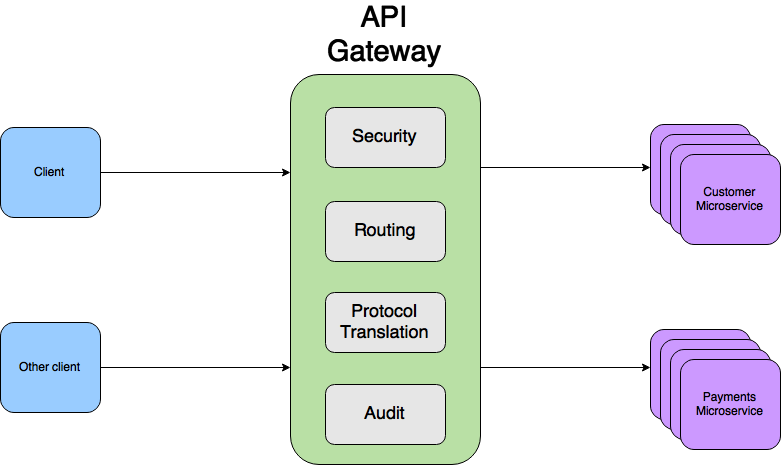
\includegraphics[scale=0.4]{images/AGARC.png}
	\caption{طرح کلی الگوی درگاه ارتباط با رابط‌های برنامه‌نویسی}
\end{figure}

\cleardoublepage 